\documentclass[aps,prb,superscriptaddress,amsmath,amssymb,showpacs,twocolumn]{revtex4}
%\documentstyle{article}
%\usepackage[paperwidth=210mm,paperheight=297mm,centering,hmargin=1.8cm,vmargin=1.8cm]{geometry}
\usepackage{amsmath}
\usepackage{graphicx}
\usepackage{amssymb}
\usepackage[usenames,dvipsnames]{xcolor}
\usepackage{subfigure}
\usepackage{dcolumn}% Align table columns on decimal point
\usepackage{bm}% bold math
\usepackage{ulem}
\usepackage{caption}
\normalem


\bibliographystyle{apsrev}
\makeatletter
\begin{document}
%opening

\title{An \textit{ad hoc} improvement to ring polymer molecular dynamics}
\author{Mariana Rossi}
\affiliation {Physical and Theoretical Chemistry Laboratory, 
University of Oxford, South Parks Road, Oxford OX1 3QZ, UK}
\author{Michele Ceriotti}
%\email{michele.ceriotti@chem.ox.ac.uk}
\affiliation {EPFL}
\author{David E. Manolopoulos}
\affiliation {Physical and Theoretical Chemistry Laboratory, 
University of Oxford, South Parks Road, Oxford OX1 3QZ, UK}


\newcommand{\avg}[1]{\ensuremath{\left<#1\right>}}
\newcommand{\mc}[1]{{\color{blue}#1}}
\newcommand{\mr}[1]{{\color{Plum}#1}}
%\newcommand{\remove}[1]{{\sout{#1}}}
\newcommand{\remove}[1]{}
\newcommand{\oxford}[1]{{\color{blue} #1}}
\newcommand{\berlin}[1]{{\color{red}#1}}
\newcommand{\Tr}{\ensuremath{\operatorname{Tr}}}
\newcommand{\img}{\ensuremath{\mathrm{i}} }
\newcommand{\diff}{\ensuremath{\mathrm{d}} }
\newcommand{\Cqq}{\ensuremath{\tilde{C}_{qq}(t) }}


\begin{abstract} 
Two of the most successful methods that are available for simulating the quantum dynamics of
condensed phase systems are ring polymer molecular dynamics (RPMD) and centroid molecular dynamics (CMD).
Despiste their conceptual differences, practical implementations of these methods differ in just two aspects:
the choice of the Parrinello-Rahman mass matrix and whether or not a thermostat is applied to the internal 
modes of the ring polymer during the dynamics. 
Here we explore a method which is in a sense `half-way' 
between the two approximations: we keep the path integral bead masses equal to the physical particle
masses but attach a path integral Langevin equation (PILE) thermostat to the internal modes of the
ring polymer. The justification for this is that the inclusion of an internal mode thermostat does
not affect any of the wholesome features of RPMD: because of the choice of bead masses, the 
resulting method is still optimum in the short-time limit, and the transition state approximation
to its reaction rate theory remains closely related to the semiclassical instanton approximation
in the deep quantum tunneling regime. In effect, there is a continuous family of methods with
these properties, parameterised by the coupling strength of the PILE thermostat,
\mc{that equally well preserve the short-time limit of RPMD, which depends on the choice of the mass
matrix but is not sensitive to thermostatting of the internal modes. }
Here we explore numerically how the approximation to quantum dynamics depends on this coupling strength, % MR: maybe not?
with a particular emphasis on vibrational spectroscopy.
\mc{We find that a broad range of values around the critical damping chosen
for the original PILE thermostat give very similar results, that give a reasonable
albeit arguably \emph{ad hoc} approximation to quantum effects, while being 
immune to both the resonance problem of RPMD and the curvature and time step problems of CMD.
\sout{We find that the critical damping chosen
for the original PILE thermostat is close to optimum, % MR: maybe we also don't need to say this.
and that the resulting dynamical approximation
is immune to both the resonance problem of RPMD and the curvature problem of CMD.}
}
\end{abstract}

\maketitle

The quantum nature of light nuclei has a very significant impact on the behaviour
of molecules and materials, not only at cryogenic temperatures, but also at room 
temperature and above. 
Well-established techniques exist to perform atomistic simulations that accurately
and rigorously include nuclear quantum effects (NQEs) on static, time-independent
configurational and thermodynamic
properties\cite{feyn-hibb65book,chan-woly81jcp,parr-rahm84jcp,cepe95rmp},
and efforts are concentrated on making them less demanding, with some success \cite{ceri-mano12prl,  SUZUKI-CHIN/TUCKERMAN} 

For what concerns dynamical properties, however, the situation is much less clear.
Exact techniques are extremely complex, and impractical for anything but the simpler
molecules~\cite{????DAVID????}. Approximate techniques are restricted to either quasi-harmonic
perturbative expansions\cite{????} or one of few approximate, semi-classical 
techniques, most notably the linearized semi-classical initial value representation (LSC-IVR),
centroid molecular dynamics (CMD)~\cite{cao-voth93jcp,cao-voth94jcp}, and ring-polymer 
molecular dynamics (RPMD).
LSC-IVR can be derived rigorously starting from quantum mechanical expressions, but 
the approximations that are practically affordable are affected by severe
zero-point energy leakage, which makes it very hard to collect satisfactory statistics
and casts shadows on the applicability to long-time properties of anharmonic systems.
CMD and RPMD both can be regarded as real-time versions of imaginary-time path integrals,
CMD being essentially classical molecular dynamics on the centroid potential of mean force,
RPMD being classical molecular dynamics based on the ring polymer Hamiltonian. 
Both are to an extent arbitrary, \emph{ad hoc} approximations, even though recent 
efforts have put them on somehow more robust grounds \cite{rich-alth09jcp,hele-alth13jcp,jangvoth99jpc, jangvoth99jpc2, MORE?}.
They are only exact for linear operators in the harmonic limit\cite{habe+13arpc, jangvoth99jpc2}, and 
both are known to exhibit artefacts that are most evident when computing vibrational
spectra of molecules~\cite{witt+09jcp, ivanov+10jpc, habe+08jcp}, that are related to the so-called curvature problem for CMD
(that we will interpret as a consequence of adiabatic separation between the centroid
and the internal modes of the ring polymer) and resonance between physical modes
of the system and internal modes of the ring polymer for RPMD.

Here we will discuss the effect of thermostatting the internal modes of the ring
polymer while using the physical ring polymer mass matrix, thereby obtaining a method
that can be regarded as a ``hybrid'' of RPMD and CMD. We will show that both 
the short-time limit accuracy of RPMD and the analogy between RPMD and the instanton
in the study of rates are not affected by the use of stochastic thermostats for the
internal modes of the  ring polymer. This means that there is a whole family of methods,
differing by the details of the thermostatting, that are not more a \emph{ad hoc}
than RPMD, and offer a way to improve upon the existing approximations. 
While we cannot at this stage suggest a way to exploit this additional
freedom to obtain a more rigorous method for quantum dynamics, we show that
for a broad range of thermostat parameters, this stochastic term
cures the resonance problem of RPMD without triggering the curvature
problem. Furthermore, this method can be ued with much larger time steps
than CMD, as it uses the RPMD mass matrix and does not rely on adiabatic separation.

The Langevin RPMD approach we introduce (which we refer to as \textit{PILE}) is a practical solution to explore
the role of NQEs on dynamical properties, even though we cannot claim that there is 
a universal choice of the damping that gives a rigorously better approximation 
to quantum dynamics. It is quite possible that by exploring the additional 
degrees of freedom that are associated with stochastic dynamics of the 
internal modes of the ring polymer future research may eventually fulfill this 
arduous goal.

\section{ALL SECTIONS FROM DAVID \label{sec:invariance}}


%\section{The resonance problem}
%
%\mc{Do we want to put the analytical results for the off-diagonal coupled oscillators here?}
%\mr{If we can show just a picture about how PILE changes the spectrum, it would be nice.}
%
%We here define the ring polymer effective Hamiltonian, in the bead representation, as
%
%\begin{eqnarray}
%H_n & = & \underbrace{\sum_i^N \sum_j^n \left[\frac{\vert {\bf p}_i^{(j)} \vert^2}{2m^{\prime}_i} + \frac{1}{2}m_i\omega_n^2 \vert {\bf q}_i^{(j)} - {\bf q}_i^{(j-1)} \vert^2 \right]}_{H_0} \nonumber \\
%& & + \sum_j V({\bf q}_1^{(j)}, ..., {\bf q}_N^{(j)}), 
%\label{eq:pimd-hamiltonian}
%\end{eqnarray}
%
%\noindent where $H_0$ is the free ring polymer Hamiltonian, $i$ runs through the $N$ particles of the physical system, $j$ runs through the $n$ path integral replicas,
%${\bf p}_i^{(j)}$ and ${\bf q}_i^{(j)}$ are the momenta and positions associated with particle $i$, replica $j$, respectively, $V$ is the physical interacting potential, and $\omega_n=nk_bT/\hbar$. We note that while $m_i$ should correspond to the physical masses of the system, there is no 
%$a priori$ requirement for the choices of $m^{\prime}_i$ in the standard PIMD formulation, since this term is just added to the Halmiltonian
%to allow the evaluation of the dynamics. Finally, ${\bf q}_i^{(n+1)} = {\bf q}_i^{(1)}$, which closes the ring polymer. 
%
%As explained in detail in Ref. \cite{ceri+10jcp}, it is possible to perform a normal mode transformation on the Hamiltonian above, such that
%the free ring polymer Hamiltonian $H_0$ can be written as
%
%\begin{eqnarray}
%H_0 & = &  \frac{1}{2}{\bf \tilde{P}}^T {\bf M}^{-1} {\bf \tilde{P}} + \sum_i^N \sum_{k=0}^{n-1} \left[ \frac{1}{2}m_i\omega_k^2 ({\bf \tilde{q}}_i^{(k)})^2 \right],
%\label{eq:h0-normalmode}
%\end{eqnarray}
%
%\noindent where $\tilde{P}$ is an array containing all normal mode transformed momenta ${\bf \tilde{p}}_i^{(k)}$, ${\bf \tilde{q}}_i^{(k)}$ are the normal mode  transformed coordinates, and $\omega_k = 2 \omega_n \sin(k\pi/n)$. In RPMD, the mass matrix ${\bf M}$ simply a diagonal matrix containing all the physical masses $m_i$ of the system, and the time evolution of position and momenta are carried out without any thermostat attached to them. In the normal mode representation, $k$=0 is the mode connected to the centroid and $k>0$ represent the internal modes of the ring polymer. It is already worth pointing out that $\omega_1 \approx 2\pi/(\beta\hbar)$ for the free ring polymer lies around 1300 cm$^{-1}$ at 300K and around 435 cm$^{-1}$ at 100K (a temperature that will be important later on in this paper).
%
%As pointed out in Refs. \cite{habe+08jcp, witt+09jcp, ceri+11jcp}, if one applies the RPMD formalism to a simple potential corresponding to a chain of uncoupled harmonic oscillators $V({\bf q})=\sum_i m_i\omega_i^2q_i^2/2$,
%it is straightforward to show that the frequencies of vibration of ring polymer will be given by \mr{check!}
%
%\begin{eqnarray}
%\omega_k^{i}=\sqrt{\omega^2_i + 4 \omega_n^2 \sin^2(k\pi/n)},
%\label{eq:harm-freq-rpmd}
%\end{eqnarray}
%
%\noindent such that the centroid vibrates at the frequencies of the physical system and the other internal modes vibrate at higher frequencies. Clearly, in any real system, the potential will not be exactly harmonic, and the expression in Eq. \ref{eq:harm-freq-rpmd} will be just an approximation for the internal frequencies of the ring polymer. Nevertheless, Eq. \ref{eq:harm-freq-rpmd} already shows clearly the origin of the so-called ``resonance-problem" of RPMD, thoroughly discussed in Refs. \cite{habe+08jcp, witt+09jcp}: For systems with vibrational frequencies $\omega_i$ spanning from small to large wavenumbers, there will be an $\omega_k$ for, e.g. a small $\omega_i$ that will have a very similar frequency to another larger $\omega_i$, so that they will resonate. The lower the temperature, the more severely will these spurious frequencies contaminate the true spectrum, so that for most real-life applications, RPMD cannot be used for the evaluation of vibrational spectra.
%
%%\mr{Show stupid plots of eq. \ref{eq:harm-freq-rpmd} for 300K and 100K with varying $\omega$ that I added to the "extra" folder?}
%
%\section{The curvature problem}
%
%The resonance problem is characteristic to RPMD. CMD avoids contamination of the 
%spectrum by internal modes of the ring polymer by (partial) adiabatic decoupling,
%that ensures that there is no overlap between the range of frequencies of the 
%centroid vibration and that of the non-zero frequency internal modes.
%On the contrary, the so-called curvature problem is characteristic of CMD, 
%and consists in a red shift of stretching modes of groups of atoms that also 
%possess librations or wagging modes, that is accompanied by a broadening of 
%the peak and that becomes more and more pronounced as the temperature decreases. 
%
%As discussed in Ref.~\cite{witt+09jcp}, the curvature problem can be understood
%as arising because the centroid moves on an effective potential, in which 
%the stretching mode is averaged over a soft, strongly non-linear 
%motion of the molecule. In fact, the curvature problem is most severe for a freely-rotating
%bond, and becomes less dramatic when the spread of the ring polymer orthogonal to
%the bond is restricted by angular restraints~\cite{witt+09jcp}, or by the presence 
%of weak interactions with other molecules~\cite{paesani-voth10jcp}.
%
%Note that one could regard this effect as a spurious coupling between
%the physical, centroid component of the stretching mode and the 
%(adiabatically decoupled) internal vibrations of the ring polymer
%in the perpendicular, free-rotation motion. There is in this regards
%an interesting connection with the resonance problem of RPMD: at 
%least in the case of the simple models discussed in Ref.~\cite{witt+09jcp}, 
%resonances happen when the \emph{free ring-polymer} internal mode frequencies 
%match the frequency of the stretching, indicating that the resonance problem
%is also exacerbated by the presence of soft, strongly non-linear wagging modes.
%
%Since the curvature problem is caused by the centroid moving on a mean 
%potential surface, averaged over the internal modes, one could 
%wonder whether thermostatting the internal modes of the ring polymer
%as we advocate here would be enough to cause a similar effect, even 
%without changing the mass matrix.
%
%
%\section{The ``PILE'' method}
%
%Since it was shown in Section \ref{sec:invariance} that the application of the PILE
%thermostat on the internal modes of the ring polymer does 
%not disturb the short time limit of RPMD \mr{(still to be shown)}, we here apply this
%technique in order to obtain vibrational spectra free of the resonances that 
%affect RPMD. We call this method \textit{PILE} in the following.
%
%As explained in Ref. \cite{ceri+10jcp}, applying the PILE thermostat amounts to
%the following equations of motion in the normal mode representation,
%
%\begin{eqnarray}
%\frac{d}{dt}{\tilde{\bf q}}_i^{(k)} & = & {\tilde{\bf p}}_i^{(k)}/m_i, \nonumber \\
%\frac{d}{dt}{\tilde{\bf p}}_i^{(k)} & = & -m_i\omega_k^2{\tilde{\bf q}}_i^{(k)} - \gamma^{(k)} {\tilde{\bf p}}_i^{(k)} + \sqrt{\frac{2m_i\gamma^{(k)}}{\beta_n}} {\boldsymbol\xi}_i^{(k)}(t),
%\end{eqnarray}
%
%\noindent where ${\boldsymbol\xi}_i^{(k)}$ is a vector of Gaussian-distributed, uncorrelated random noise. 
%The $\gamma^{(k)}$ friction coefficients that yield critical damping are the ones that minimize
%the correlation time $\tau_H$ for the Hamiltonian of the harmonic oscillator, subject to the Langevin equations of
%motion above. As explained in Ref. \cite{ceri+10jcp}, the analytical result is,
%
%\begin{equation}
%\tau_H=\frac{1}{\gamma^{(k)}} + \frac{\gamma^{(k)}}{4\omega_k^2},
%\end{equation} 
%
%\noindent so that the optimum value is $\gamma^{(k)}_c=2\omega_k$. The difference of the treatment here,
%as compared to the one in Ref. \cite{ceri+10jcp} is that we do set $\gamma^0=0$, i.e., the centroid mode
%is not thermostatted and follows Hamiltonian dynamics. 
%
%As shown in Section \ref{sec:invariance}, we do not find a criterion to fix the $\gamma^{(k)}$ parameters.
%While choosing them to yield critical damping seems a sensible choice, we also investigate the effect of
%changing these parameters to yield underdamped and overdamped regimes of the Langevin equation in the
%following sections.
%
%\section{The quartic oscillator}
%
%
%In this section, we show the results we obtain when applying RPMD, CMD, and the \textit{PILE} method 
%to the one dimensional anharmonic quartic potential $V(q)=q^4/4$, already explored previously in the literature (e.g. Refs. \cite{crai-mano04jcp, jangvoth99jpc}).
%We here consider $\hbar=1$, $m=1$, and $\beta=10$, in natural units. For the RPMD and \textit{PILE} simulations, we used 64 beads, and a time step $\Delta t = 0.01$ for the integrator, which ensures convergence and accuracy of all relevant quantities in the simulation. For CMD, we used a time step of 0.002 natural units.
%\mr{[comment: change PILE for \textit{PILE} in the following?]}
%
%\begin{figure}[htbp]
%\begin{center}
%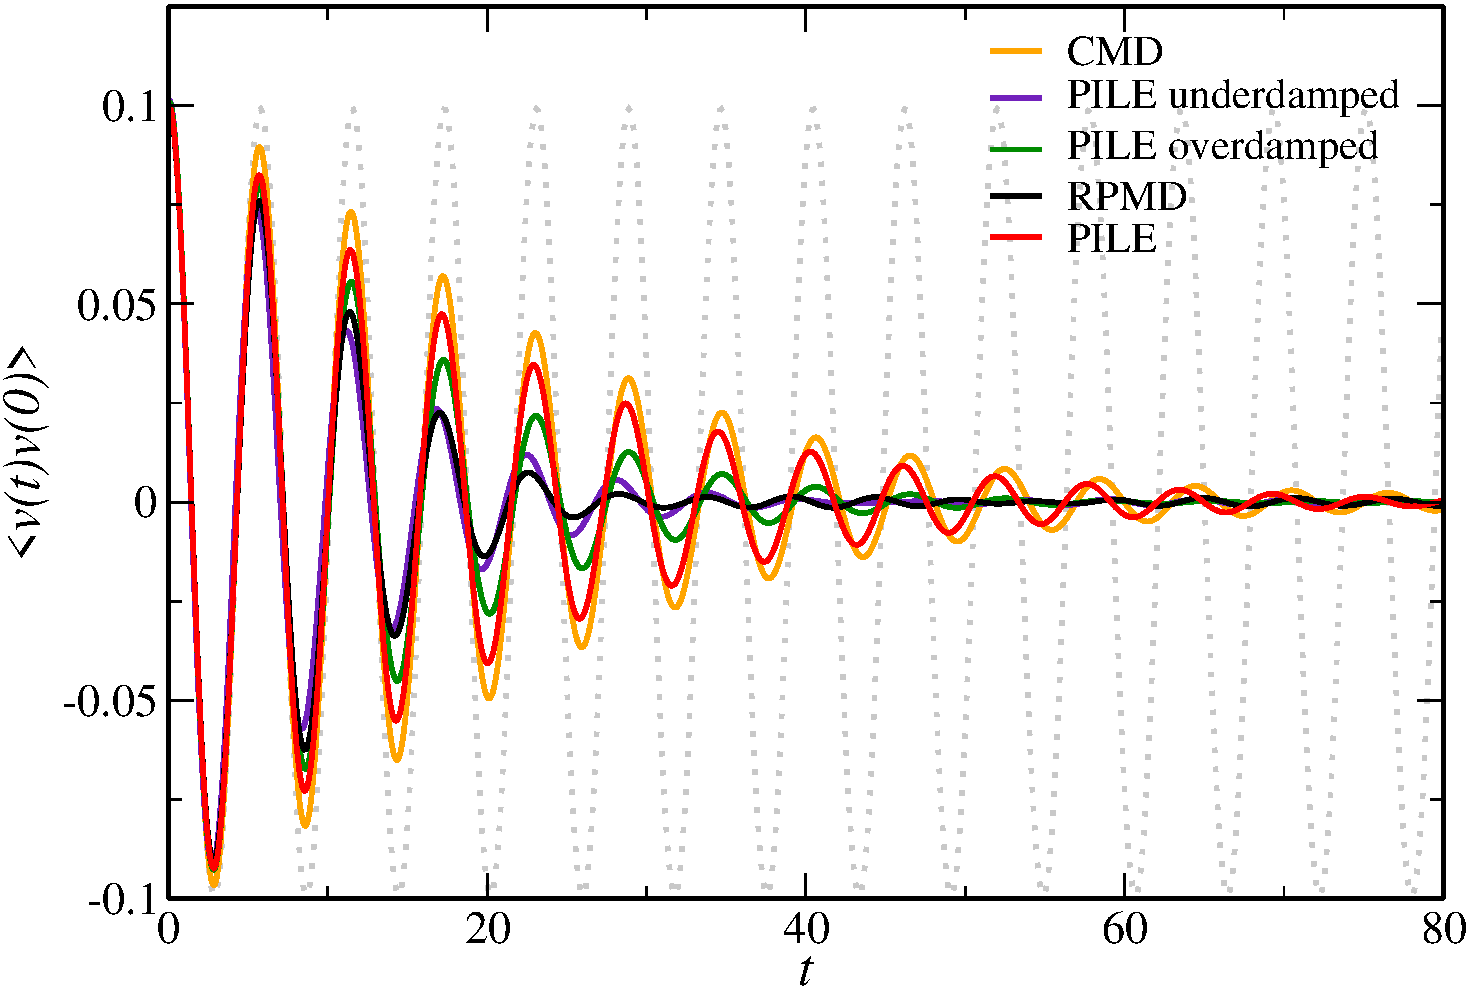
\includegraphics[width=0.48\textwidth]{figures/vv_autocorr_quartic}
%\end{center}
%\caption{Velocity autocorrelation function for the quartic one-dimensional potential $V(q)=q^4/4$. The dotted line corresponds to the exact result. All units are atomic units, $m$=1, and $\beta$=10.}
%\label{fig:autocorr-quartic}
%\end{figure}
%
%In Figure \ref{fig:autocorr-quartic}, we show the velocity autocorrelation functions calculated from 10000 trajectories of 200 time units. 
%All correlation functions were obtained after thermalization runs with a simple Andersen thermostat. We plot the correlation function of RPMD, CMD,
%PILE ($\gamma^{(k)}=\gamma^{(k)}_c$), underdamped PILE ($\gamma^{(k)}=0.1\gamma^{(k)}_c$), and overdamped PILE ($\gamma^{(k)}=10\gamma^{(k)}_c$). The dotted lines correspond to the
%exact result, in which the autocorrelation function does not decay. All methods predict an artificial decorrelation of the autocorellation function, with CMD being the closest to the exact result and PILE (critical damping), being the second best. The fact that critically damped PILE gives a better result
%than RPMD and than its underdamped and overdamped variations is not expected to be always true - it just happens to be the
%case for this potential. In any case, what we do expect, given the mathematical derivations above, is that PILE still gives a good approximation
%to the real quantum result in a wide range of systems.
%
%\begin{figure}[htbp]
%\begin{center}
%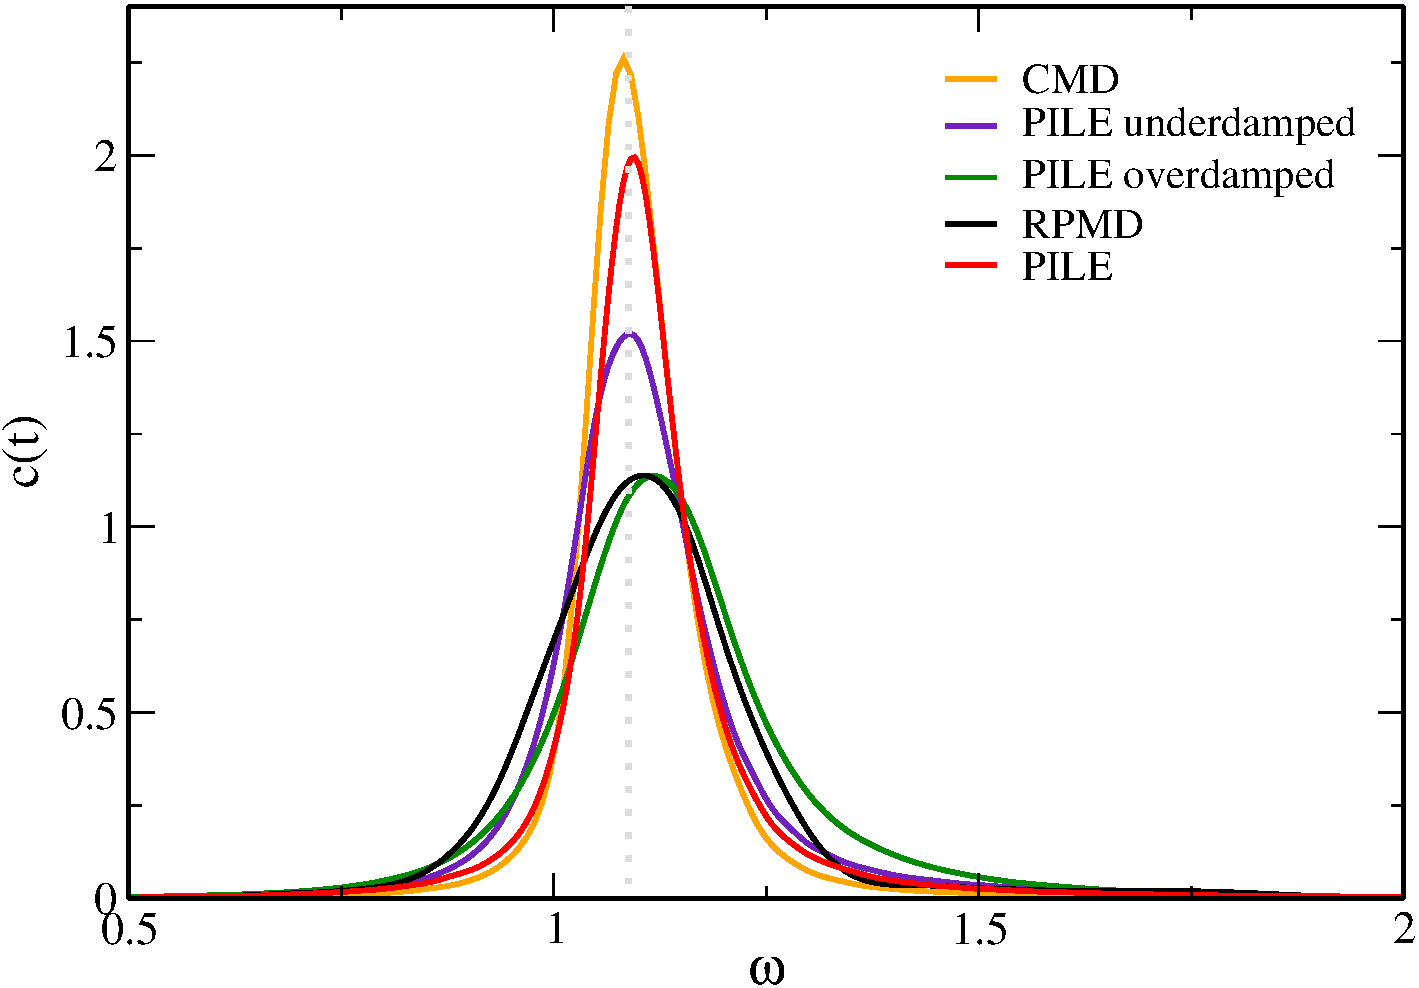
\includegraphics[width=0.38\textwidth]{figures/vv_fourier_quartic.pdf}
%\end{center}
%\caption{Fourier transform of the velocity autocorrelation function for the quartic one-dimensional potential $V(q)=q^4/4$. The dotted line corresponds to the expected exact result for the position of the peak. All units are atomic units, $m$=1, and $\beta$=10.}
%\label{fig:spec-quartic}
%\end{figure}
%
%
%We note that for this 1D potential there will be no resonance problem in RPMD in the main peak, since the ring-polymer frequencies are always shifted to higher frequencies with respect to the first physical one ($\approx$ Eq. \ref{eq:harm-freq-rpmd}), and there is only one frequencies. We see this effect in the overtones but since they have very low intensity, they do not affect the spectrum. Also, there is no curvature problem, simply because it is a 1D potential. In Figure 
%\ref{fig:spec-quartic} the corresponding Fourier transforms of the autocorrelation functions shown in Fig. \ref{fig:autocorr-quartic} are shown, which just confirm the considerations above. CMD and critically damped PILE produce the narrowest peaks, with the exact result being a $\delta$-function centered at the position of the dotted line. 

\section{Solving the resonance and curvature problems}

In the previous section we have demonstrated that adding a stochastic thermostat to the internal degrees of freedom
of a ring polymer without changing the mass matrix preserves all of the wholesome properties of RPMD, and only reduces
the short-time limit accuracy by one order in time. In Ref.~\cite{witt+09jcp} it was shown that both RPMD and CMD 
exhibits clearly unphysical artefacts when it comes to modeling infra-red spectroscopy and vibrational dynamics. 
Namely, vibrational spectra obtained by RPMD are contaminated by resonances between the physical vibrational modes
of the system and the internal modes of the ring polymer, whyle CMD spectra are affected by a curvature problem that
causes high frequency peaks to broaden and shift to lower frequencies with decreasing temperature. 

\begin{figure}[htbp]
\centering
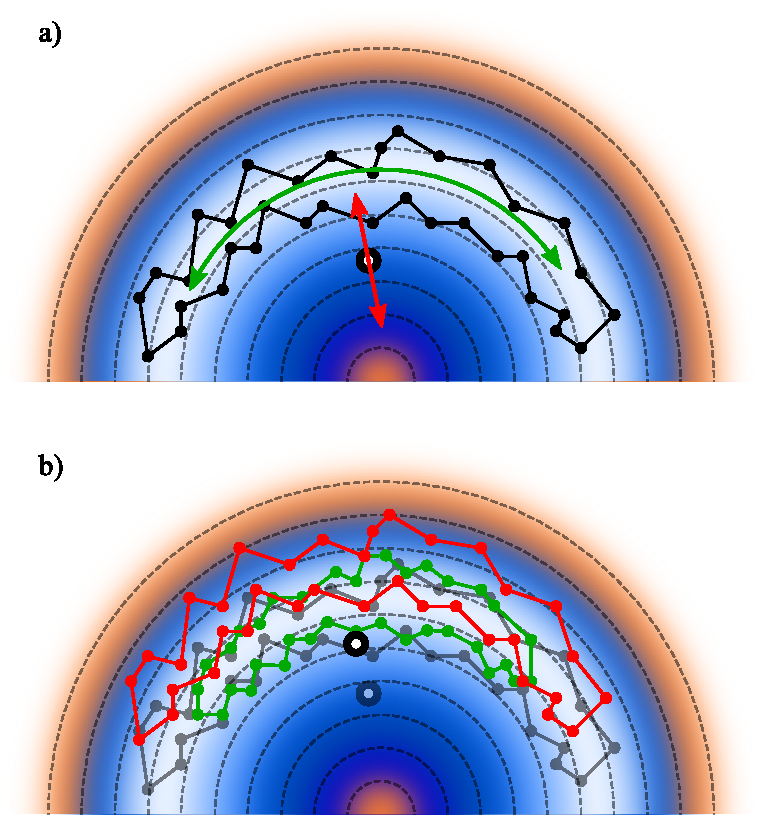
\includegraphics[width=0.5\textwidth]{figures/champagne.pdf}
\caption{Schematic representation of the source of the resonance and curvature problems for a ring polymer 
moving on top of a champagne-bottle potential (represented by the color scale, where white represents low energy and blue 
and orange higher energies). a) Internal motion of the ring polymer in the angular direction can couple with motion 
of the centroid in the radial direction. b) When internal motion of the ring polymer is decoupled from the centroid, 
the ring polymer can relax the energy by contracting or relaxing in the angular direction, effectively softening the
potential of mean force in the radial direction. }
\label{fig:champagne}
\end{figure}

Both of these problems are two faces of the same coin, and can be traced to the interplay of 
high-frequency stretching modes and near-zero frequency rotations or wagging modes of the bond. 
 This can be understood by considering a ring polymer in a ``champagne bottle'' potential, as in 
Figure~\ref{fig:champagne}a. Internal vibrations of the ring polymer along the angular direction 
engender a net motion of the centroid in the radial direction, which is amplified
when the two motions are in resonance. In the presence of a harmonic potential of frequency $\omega$, 
the ring polymer frequencies are shifted to $\sqrt{\omega^2 + \tilde{\omega}^2_k}$, so in a truly 
one-dimensional system there can never be a resonance. The fact that resonances involve an interplay 
of different physical directions is apparent from the fact that they are observed when \emph{free ring polymer} 
frequencies overlap with the range of frequencies corresponding to physical vibrational frequencies.

The adiabatic decoupling that underlies CMD can shift the internal vibrations outside of the range of 
physical frequencies, but does not eliminate the fact that internal angular vibrations are geometrically 
coupled with the radial centroid motion. 
As shown in Figure~\ref{fig:champagne}b, a radial displacement of the ring polymer that would correspond to a high 
curvature of the potential can also be produced by an internal contraction in the soft angular
direction. This results in an effective softening of the radial potential of mean force, which is the essence
of the curvature problem as discussed in Ref.~\cite{witt+09jcp}.


\subsection{Model molecules: OH and CH$_4$}

\begin{itemize}
\item Remove parameters that are already in Marx paper -- just refer to it
\item Introduce IR spectrum as discussed with David
\item Discuss the two molecules at the same time -- they are the same, just say
that CH4 shows less of the curvature problem as discussed in the OTHER Marx paper. 
Say that RPMD resonances are not healed by an angular potential because they are related
to vibrations as opposed to relaxation of the ring polymer as in CMD curvature problem
\item Real OH -- as in Marx discuss the problem where you can't tell the anharmonic shift from
the curvature problem in CMD, show that PILE is nearly on top of the anharmonic shift. Do a figure with the peak
position and amplitude as a function of T for PILE and CMD -- not RPMD where there are multiple peaks.
\item Zundel -- real potential, complex features, note that the doublet which is genuinely quantum 
cannot ever be reproduced by semiclassical methods.
\end{itemize}



We start by studying two model molecules that have been studied in Ref. \cite{witt+09jcp},
namely the OH and the CH$_4$ molecules with an interatomic potential given by

\begin{equation}
\phi=\sum_{bonds} \frac{k_b}{2} (r-r_{eq})^2 + \sum_{angles} \frac{k_a}{2}(\theta - \theta_{eq})^2,
\end{equation}

\noindent where we use all the same values for $k_b$, $k_a$, $r_{eq}$, and $\theta_{eq}$ that were used in Ref. \cite{witt+09jcp}.
%These model molecules are especially interesting because they are known cases where
%both the curvature and the resonance problems have been well studied by Witt and coworkers\cite{witt+09jcp}.
%As in Ref. \cite{witt+09jcp}, we chose $k_b=0.49536$ Ha/bohr$^2$ and $r_{eq}=1.0$\AA~ for the OH molecule,
%and  $k_b=0.30345$ Ha/bohr$^2$, $k_a=3.1068\times10^{-5}$ Ha/deg$^2$, $r_{eq}=1.09$\AA, and $\theta_{eq}=107.8$deg for
%the CH$_4$ molecule. 

\begin{figure}[htbp]
\centering
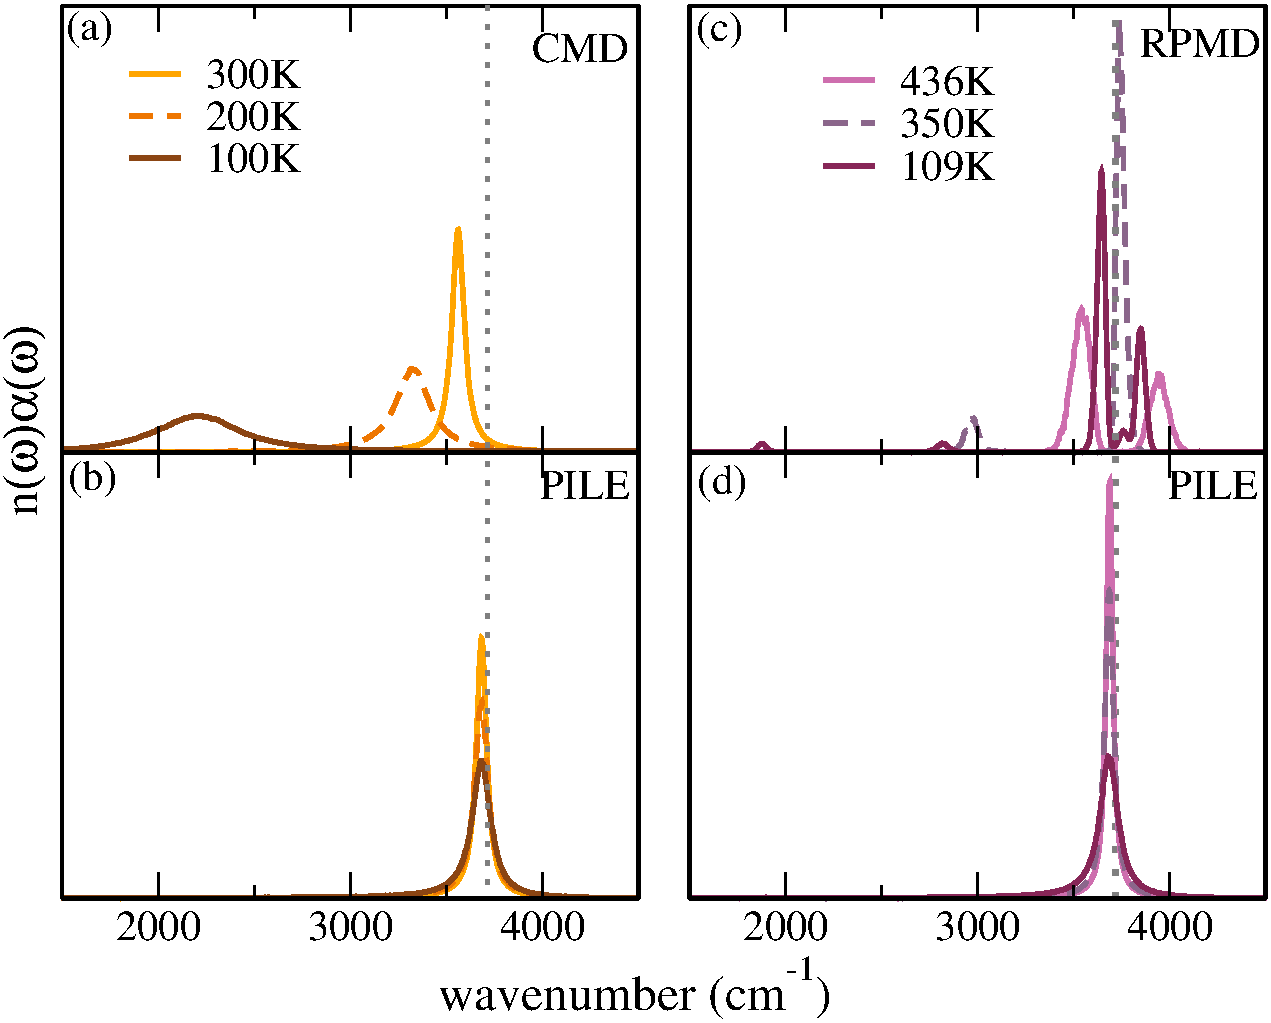
\includegraphics[width=0.5\textwidth]{figures/comparison_oh_factors.pdf}
\caption{Dipole absorption cross section for the OH model molecule: (a) and (b) CMD and PILE methods at 100, 200, and 300K ; (c)  and (d) RPMD and PILE methods at 109, 450, and 436 K. The dotted grey line corresponds to the classical vibrational frequency predicted for this model.}
\label{fig:oh-rpmd-cmd-pile}
\end{figure}

\begin{figure}[htbp]
\centering
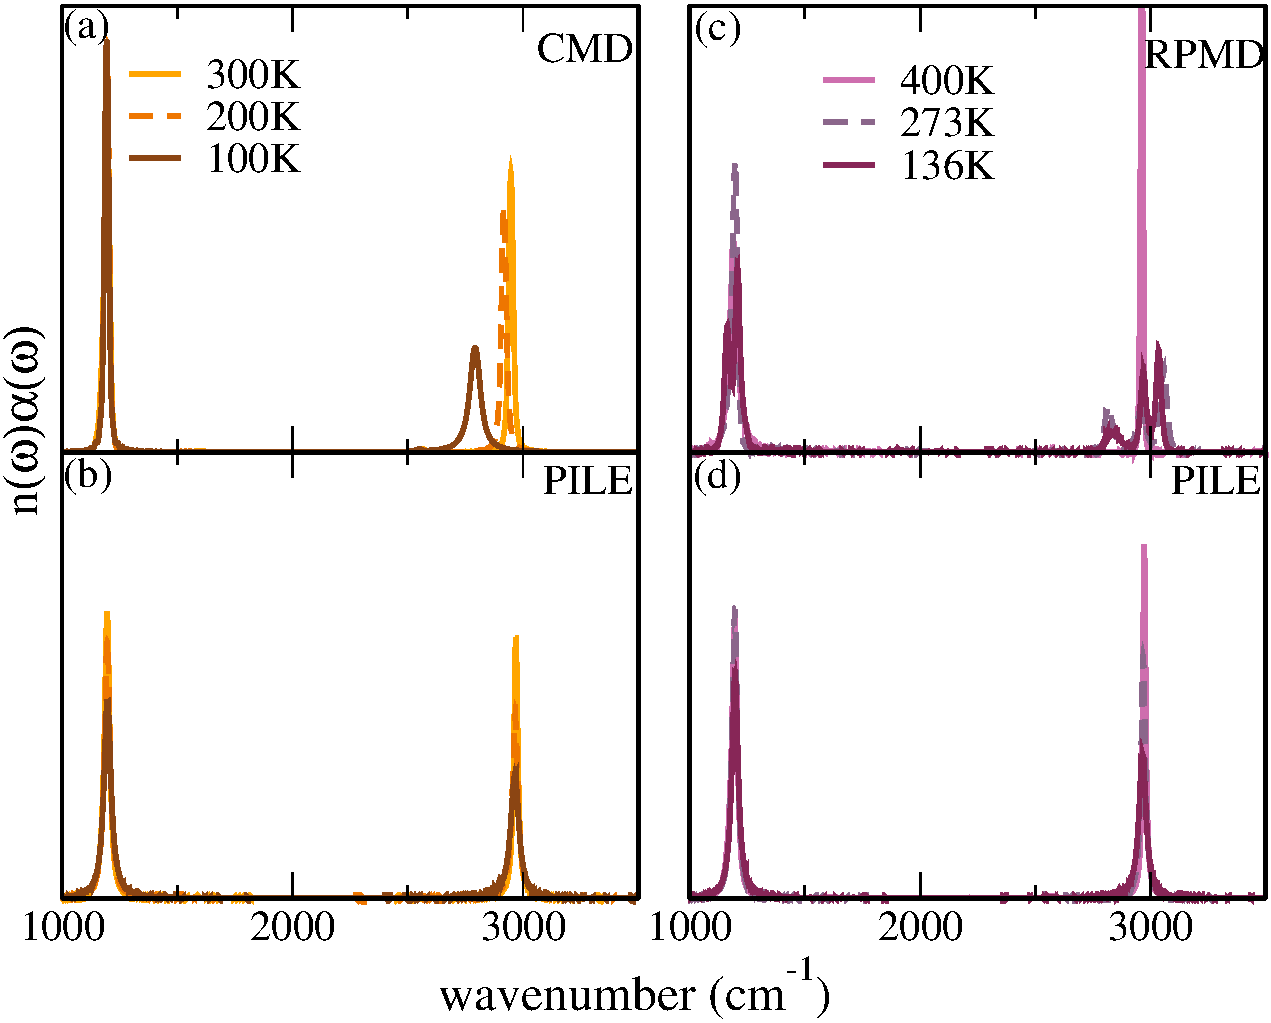
\includegraphics[width=0.5\textwidth]{figures/comparison_ch4_factors.pdf}
\caption{Dipole absorption cross section for the CH$_4$ model molecule: (a) and (b) CMD and PILE methods at 100, 200, and 300K; (c) and (d) RPMD and PILE methods at 136, 273, and 450 K.}
\label{fig:ch4-rpmd-cmd-pile}
\end{figure}

For these models, we calculate the dipole absorption cross section $n(\omega)\alpha(\omega)$, which is proportional to 

\begin{equation}
n(\omega)\alpha(\omega) \propto \omega^2  \tilde{I}(\omega),
\end{equation}

\noindent where $\tilde{I}(\omega)$ is the Fourier transform of the Kubo-transformed dipole autocorrelation function.
It is this autocorrelation function that we approximate with CMD, RPMD, and the PILE method. We here also filter out
translations and rotations of the molecule using the scheme proposed in Ref. \cite{witt+09jcp}.


For  both molecules we calculate the spectra at the same temperatures and with the same number of beads used in Ref. \cite{witt+09jcp}.  
%namely 109 K and 64 beads (resonant case), 350K and 16 beads (non-resonant case), and 436K and 16 beads (resonant case). We used a time
%step of 0.25 fs for these simulations.
In Figures \ref{fig:oh-rpmd-cmd-pile} and \ref{fig:ch4-rpmd-cmd-pile} we show 
in panels (a) and (c) the CMD and RPMD 
spectra for the OH and CH$_4$ molecules, respectively.
For the OH molecule, we show a dotted line where the
exact frequency of vibration should be (3715.6 cm$^{-1}$). 
The results show that the curvature problem of CMD is more 
accentuated for the OH molecule than for the CH$_4$ molecule: in
both cases the peaks at $\approx$ 3000cm$^{-1}$ shift (quite dramatically)
to lower frequencies and broaden substantially. 
For RPMD, the resonances with the internal modes of the ring polymer
split the vibrational peaks at the resonant temperatures (109K and 436K for
OH and 136K and 273K for CH$_4$). In panels (b) and (d) of Figures  \ref{fig:oh-rpmd-cmd-pile} and \ref{fig:ch4-rpmd-cmd-pile} we show the PILE results for the corresponding temperatures of the OH and CH$_4$ molecules
respectively. In all cases the resonant frequencies disappear and the curvature problem is not present. 
This shows that the curvature problem is indeed a feature of the choice
of the mass matrix used in CMD (in order to adiabatically separate the 
internal modes of the ring polymer from the centroid), 
and not related to the thermostatting of the internal modes.
We note, nevertheless, that the PILE
spectrum gets slightly broader as the temperature is lowered. 
This effect arises from the fact that at lower
temperatures there are more internal frequencies of the
 ring polymer which interact with the physical frequency.
 As will be further discussed in the next section, all
 of these methods introduce an artificial broadening in the vibrational spectrum.

\begin{figure}[htbp]
\centering
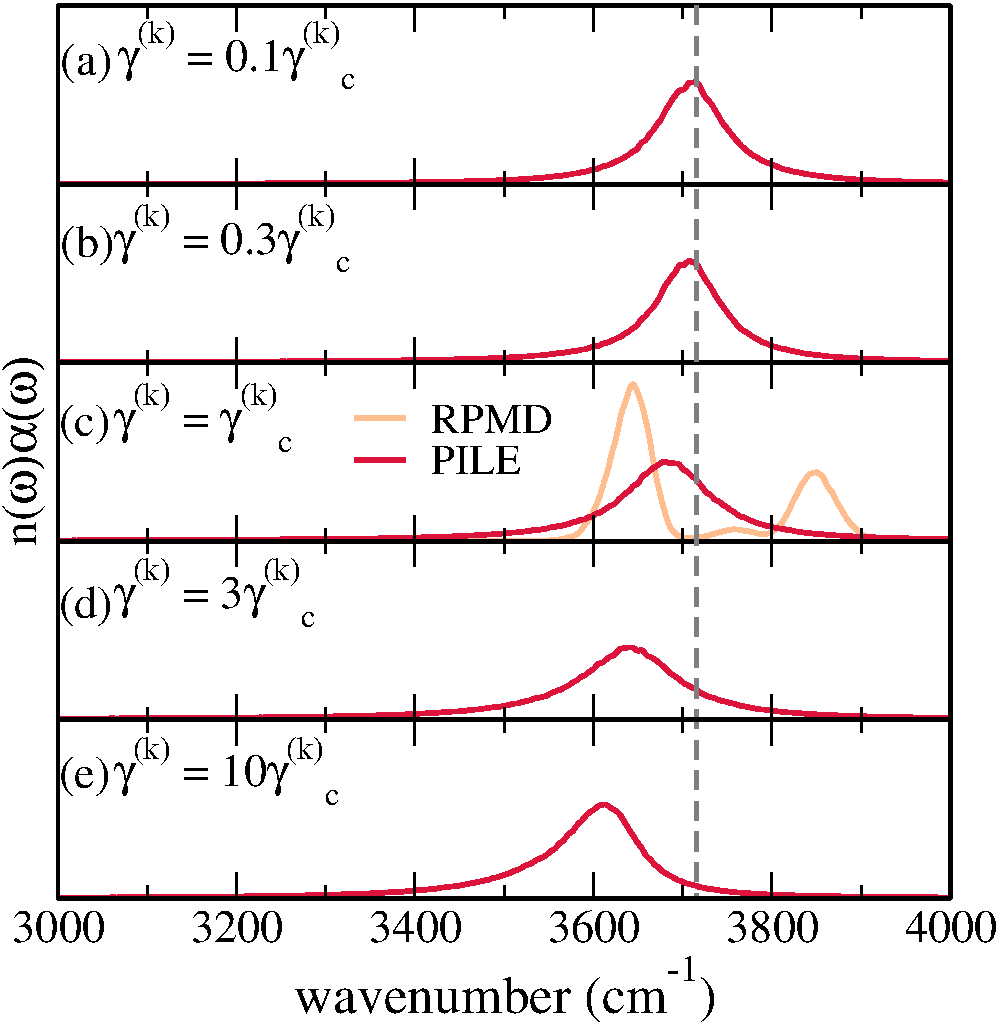
\includegraphics[width=0.4\textwidth]{figures/oh_rpmdvspiledampings_109K.pdf}
\caption{Dipole absorption cross section for the OH model molecule at 109K. The various plots show the RPMD spectrum compared to the PILE methods with different $\gamma^{(k)}$ parameters.}
\label{fig:oh-rpmd-pile-dampings}
\end{figure}

For the purpose of investigating the effect that the $\gamma^{(k)}$ parameters
have on the position and broadening of the vibrational peaks, we show in
Figure \ref{fig:oh-rpmd-pile-dampings} the
PILE IR spectrum of the OH molecule at 109K calculated with different
$\gamma^{(k)}$ parameters both in the underdamped and overdamped regimes. 
The changes observed are not substantial: Going as high as ten times the critical damping, or as low
as one tenth of it, does not change the peak position by more than 3\% of its wavenumber. Since we do not
find a mathematical criterion to fix these parameters, this uncertainty is  intrinsic to this method.



\section{Real OH}

We consider the real OH molecule with the interatomic potential given by a Morse-type potential of the form

\begin{equation}
\phi = D_{e} \left[ 1-e^{-\alpha(r-r_{e})}\right]^2 
\end{equation}

\noindent where $D_{e} = \omega_e^2/4\omega_e\chi_e$, $\alpha=\sqrt{2\mu_{OH}\omega_e\chi_e}$. The parameters $\omega_e$=3737.76 cm$^{-1}$, $\omega_e \chi_e$=84.881 cm$^{-1}$, and $r_{e}$ = 0.96966 \AA\, were obtained from the parameters measured for the real OH molecule, as reported in Ref. [HERZBERG].

\begin{figure}[htbp]
\centering
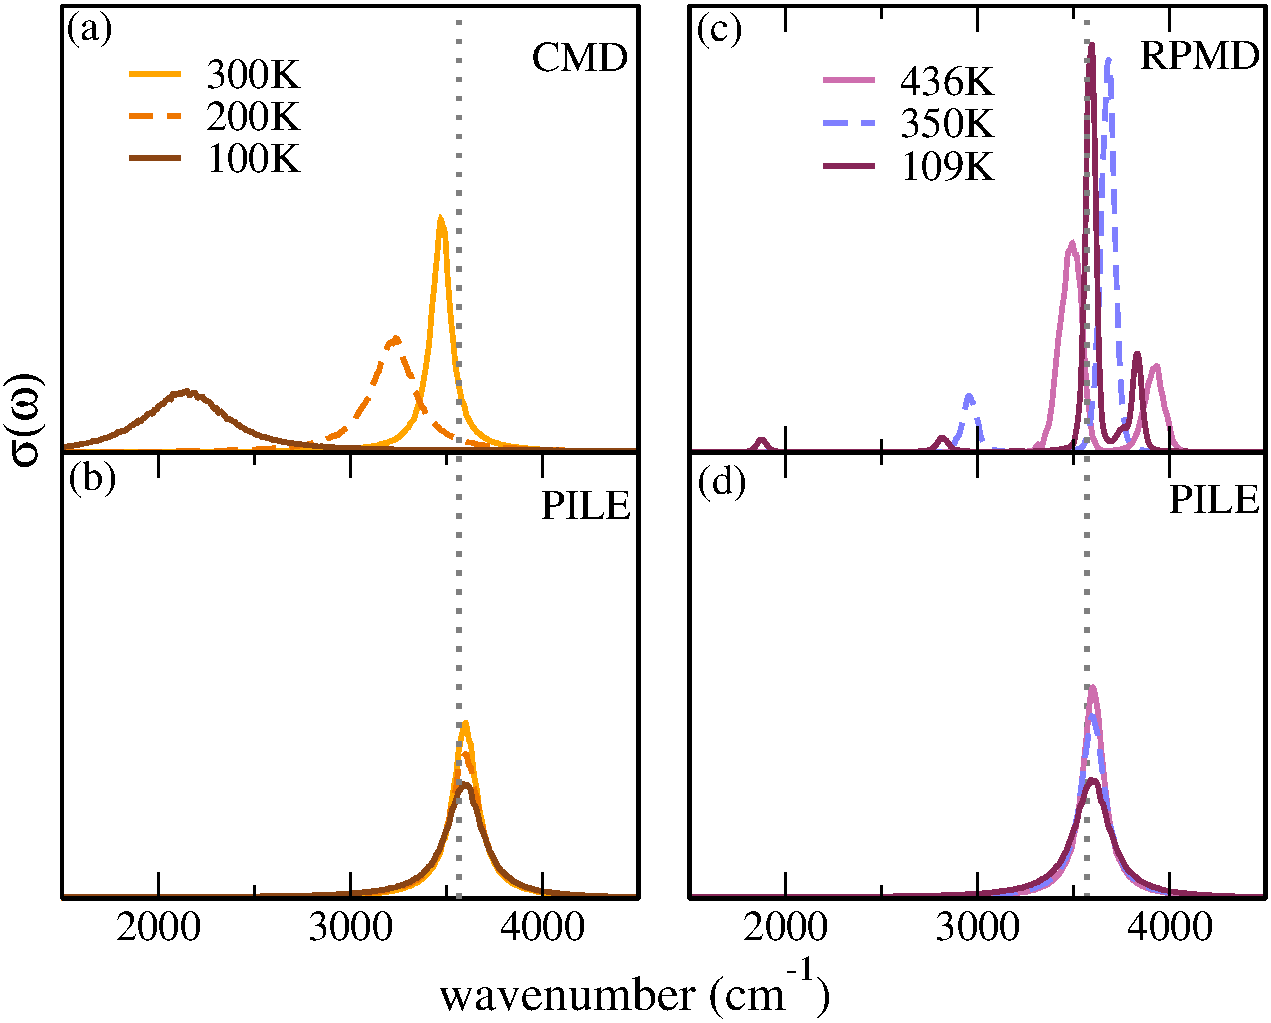
\includegraphics[width=0.5\textwidth]{figures/comparison_ohanharm_factors.pdf}
\caption{Dipole absorption cross section for the real OH molecule: (a) and (b) CMD and PILE methods at 100, 200, and 300K ; (c)  and (d) RPMD and PILE methods at 109, 450, and 436 K. The dotted grey line corresponds to the anharmonic (exact) vibrational frequency predicted for this model.}
\label{fig:oh-rpmd-cmd-pile}
\end{figure}


\subsection{The Zundel cation}

\begin{figure}[htbp]
\begin{center}
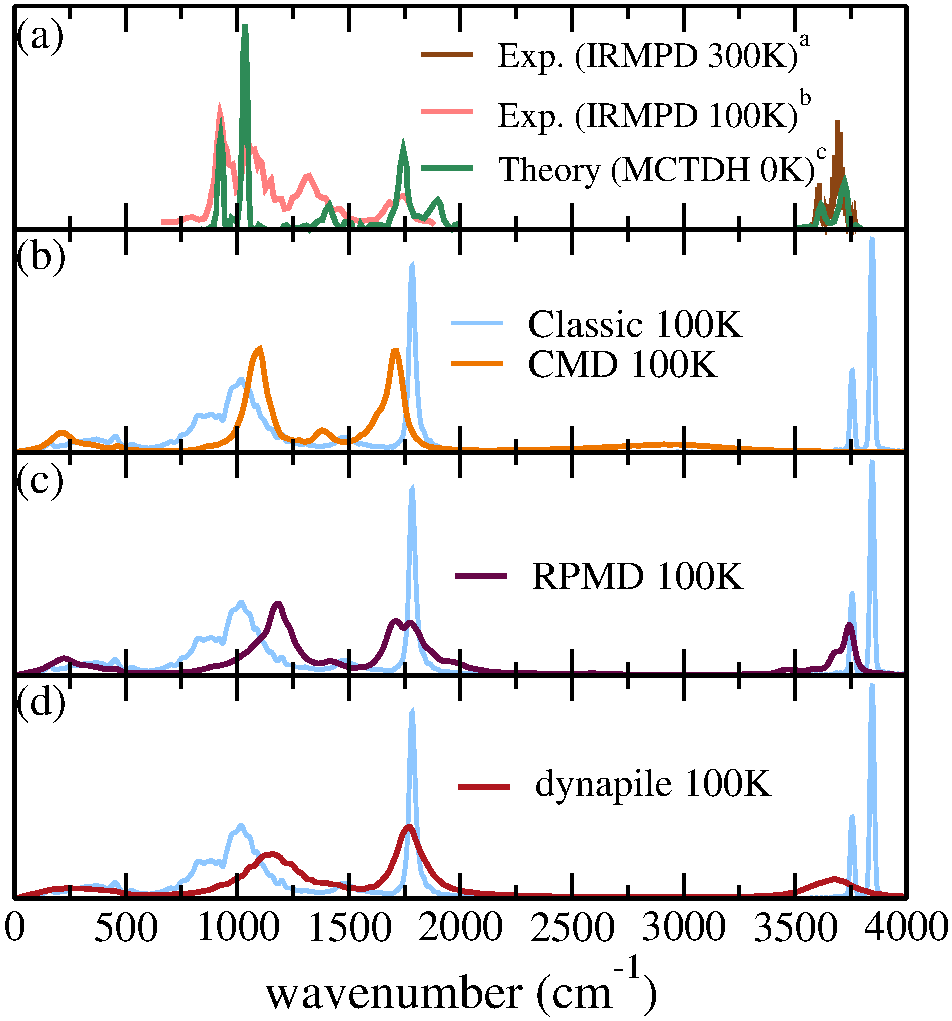
\includegraphics[width=0.48\textwidth]{figures/zundel_cleanrot_cmd_rpmd_pile.pdf}
\end{center}
{\small {}$^a$ Ref. \cite{YehLee1989}; {}$^b$ Ref. \cite{AsmisScience2003}; {}$^c$ Ref. \cite{VendrellMeyer2007}}
\caption{(a) Reference data for the IR spectrum of H$_5$O$_2^+$ taken from the literature: experimental
IRMPD data for the OH-stretch region at 300K from Ref. \cite{YehLee1989}, experimental IRMPD data between 650 and 1900 cm$^{-1}$ 
at 100K from Ref. \cite{AsmisScience2003}, and theoretical multi configuration time dependent Hartree (MCTDH) spectrum at 0K from Ref. \cite{VendrellMeyer2007}.
IR spectrum of H$_5$O$_2^+$ obtained from the Fourier transform of the dipole autocorrelation from molecular 
dynamics trajectories in the CCSD(T) parameterised surface of Ref. \cite{HuangBraamsBowman2005}, at $T$=100K: 
(b) Comparison between CMD and classical spectra, where the curvature problem is clear especially for the OH stretch peaks; 
(c) Comparison between RPMD and classical spectra, where the resonances can be seen at all peaks above 1500 cm$^{-1}$; (c)
Comparison between PILE and classical spectra, where both of the problems mentioned in (a) and (b) are not present, but the peaks
are much broader. In (d), substantial shifts due to NQE in the evaluation of the spectra can be identified.}
\label{fig:zundel-spectra}
\end{figure}


As a final example of the application of a stochastic term to remove unphysical resonances 
from RPMD spectra, let us consider a more realistic example, that also exhibits quantum
features that one cannot hope to capture with a semi-classical approach. 
The Zundel cation H$_5$O$_2^+$ is an ideal benchmark system, having been 
extensively studied in the literature~\cite{Schatteburg2008}, both theoretically 
\cite{AgostiniCiccotti2011, ParkKim2007, VenerSauer2001, SauerDoebler2005, ChengKrause1997, VendrellMeyer2007, 
BaerMarxMathias2010, KaledinBowmanJordan2009, HuangBraamsBowman2005} 
and experimentally~\cite{YehLee1989, GuascoJohnson2011, AsmisScience2003, HammerBowmanCarter2005, FridgenMaitre2004}. 
Particular attention has been given to a doublet structure in the 
shared proton stretch region that can be measured
at low temperatures~\cite{GuascoJohnson2011, HammerBowmanCarter2005}.
Theoretically,  this structure can only be captured by certain levels of 
theory that include anharmonic effects and a fully quantum mechanical treatment
of nuclear dynamics, such as the multi-configutarional time-dependent Hartree (MCTDH) method at
0K \cite{VendrellMeyer2007}. It is completely absent from any harmonic treatment,
and also expected to be absent from the methods used here due to the lack
of quantum phase information in any of them.
The Zundel cation is also convenient as a benchmark of new methodologies
because of the availability of a potential energy and dipole surfaces parametrized
with CCSD(T) data that was published by Huang, Braams and Bowman~\cite{HuangBraamsBowman2005},
which is both very accurate and inexpensive to evaluate. 


Let us first consider the frequency range corresponding to the OH stretch (Figure~???). Experiments
show two distinct peaks at about 3600 and 3700 cm$^{-1}$~\cite{YehLee1989}. As for the 
anharmonic OH discussed in the previous paragraph, the classical spectrum is blue shifted by almost 
150~cm$^{-1}$. The RPMD spectrum is closer to experiment, but shows multiple peaks and a broad
low-frequency feature. In a multi-dimensional problem such as this, resonances may be due to 
internal modes corresponding to non-zero frequency molecular vibrations which makes it hard
to predict whether or not the spectrum is contaminated by spurious oscillations. 
CMD is red shifted with respect to experiment, and does not show recognizable separate peaks.
Given the high accuracy of the potential energy surface, we can attribute the red shift to the
curvature problem -- and in fact the shift is exacerbated if the temperature is further reduced. 
As pointed out in previous work~\ref{Ivanonv????}, in a more complex case in which one could not
profit of a potential energy surface of such exquisite quality, or in the absence of very clean 
experiments, it would be impossible to determine whether the shift relative to the classical
simulation is due to genuine quantum anharmonic effects or to the artefacts of the simulation.
Finally, the position of the stretching peak in the PILE spectrum is in better agreement
with experiment, even though the excessive broadening that was also observed for the harmonic and anharmonic
OH washes out the doublet structure and yields a single, very broad peak.

Experimental data in the intermediate frequency region of the spectrum are available
from experiments at 100K~\cite{AsmisScience2003} and from highly accurate MCTDF calculations
at 0K~\cite{VendrellMeyer2007}. We performed simulations at 100K with the various methods
(Figure~????). The peaks are very broad in all cases, and RPMD 
displays multiple peaks in the bending region that can probably be attributed to resonances.
Interestingly, the bending peak for CMD is slightly lower than both experiment and MCTDH,
suggesting that at such low temperatures artefacts due to adiabatic decoupling can also manifest 
themselves for lower frequency modes than the stretches. 
None of the approximate methods investigated here can reproduce the
doublet peak at around 1000 cm$^{-1}$, which is shown in Fig. \ref{fig:zundel-spectra}(a).
Given that this doublet structure has been interpreted as a Fermi resonance
involving a fourth-order coupling between the proton transfer mode,
the O-O stretching mode, and the H-O-H wagging mode \cite{VendrellMeyer2007, Schatteburg2008},
it does not come as a surprise that it is not present in the methods investigated here:
none of these methods contain the necessary physics to describe such a resonance.

????
However, only extremely computationally expensive methods [CITE?] are able to describe
such effects, which also become less important as the system size grows. In the realm
of approximate methods for including nuclear quantum effects for dynamical observables,
and that can be applied for systems of high dimensionality without an extreme
computational cost, the newly proposed PILE method
thus emerges as the most promising candidate. 



\section{Conclusions}








\bibliography{biblio}
\end{document}
